\documentclass[10pt,a4paper]{report}
\usepackage[utf8]{inputenc}
\usepackage[english]{babel}
\usepackage{amsmath}
\usepackage{amsfonts}
\usepackage{amssymb}
\usepackage{graphicx}
\author{Gérard Tio Nogueras}
\title{Foundation Papers}
\begin{document}
\chapter{M-Trends 2015 Report}
\section{Intro}
\subsection{Targets}
Retailers are the main targets, because of their potential credentials possession.\\
New emergent target:  business and professional services, healthcare, and government and international organisations.\\
\subsection{Detection}
Surprisingly only 30 percent of the victims discover the breach internally, 70 percent are notified by external entities.
\subsection{Phising}
78 percent of phising impersonate an IT department. and 70 percent of those mails were sent between Tuesday and Friday.
\section{Trends}
\subsection{Struggling with disclosure(act of making something known)}
 More victims are publicly disclosing breaches and finding 
themselves in the media spotlight. The press, customers, and partners are 
beginning to realise that security breaches are inevitable. But at the same time, they are demanding more information and asking more detailed questions. To prepare, organisations need an effective communication strategy. The best 
strategies are guided and informed by facts determined from a thorough 
investigation of the incident.
\subsubsection{Steps of an investigation}
Questions we should ask ourselves when conducting an investigation:\\
\begin{itemize}
\item How did they get access ?
\item How did they maintain access?
\item Storyline of the attack ?
\item What data has been stolen ?
\item Is the incident contained ?
\end{itemize}
\subsection{Retail in the crosshairs}
(running the gamut = to include everything within a group or type)
Many application run on virtual machines which should make it impossible for attackers to gain access to the main server, but a slight error in the configuration can leave gaps. \\
Even if chip and PIN authentication should make it more difficult for attackers, the attacks against the technologies have increased.
\subsubsection{Case Study: 1 attacker, millions of credit cards}
Entering remotely a VM with credentials acquired priorly to the attack. Escalating privileges thanks to a misconfiguration and accessing system, using a windows FTP to dl password dumping tool,escalating to root privileges, same admin access for the whole environment.\\
(Amid = Parmi)\\
Recommendation:\\
\begin{itemize}
\item secure remote access(2 way authentification + monitoring of logons)
\item secure access to PCI(payment card inductry) environment
\item deploy app-whitelisting on critical assets
\item Manage privilege accounts
\end{itemize}
Where money goes, criminals will follow. Retailers have 
always been in the crosshairs of financially motivated cyber criminals. We saw no 
change to this in 2014. While attackers used some new techniques and grabbed 
more headlines, their playbook remained largely consistent with what we have 
observed over the last few years.\\
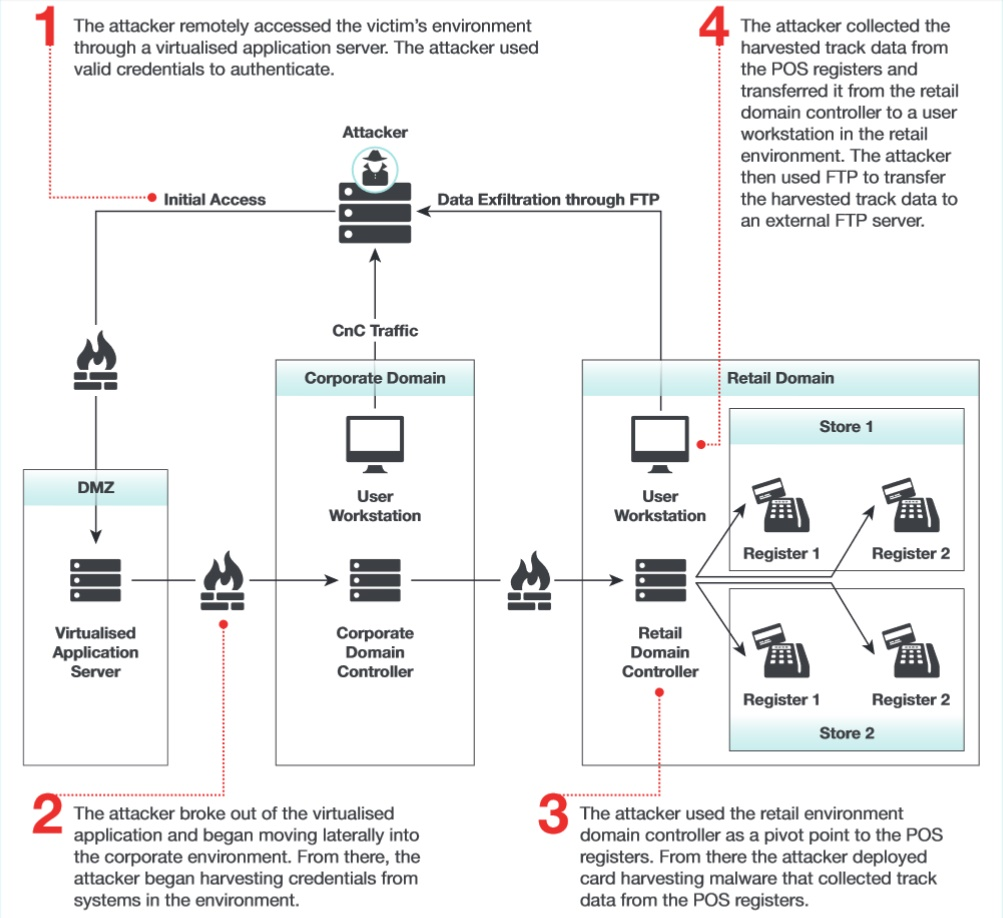
\includegraphics[scale=0.5]{caseStudy.jpg}
\subsection{The evolving attack lifecycle}
Hijacking VPN, huge grow of interest for the VPN's, and here are the 2 methods used to acquire this access:\\
\begin{itemize}
\item Single factor authentication (reuse of stolen usernames/passwords)
\item Certificate-based two-factor 
authentication: tools are used to extract the Certificates or obtained by careless exchange of these.
\end{itemize}
Here is the usual cycle\\
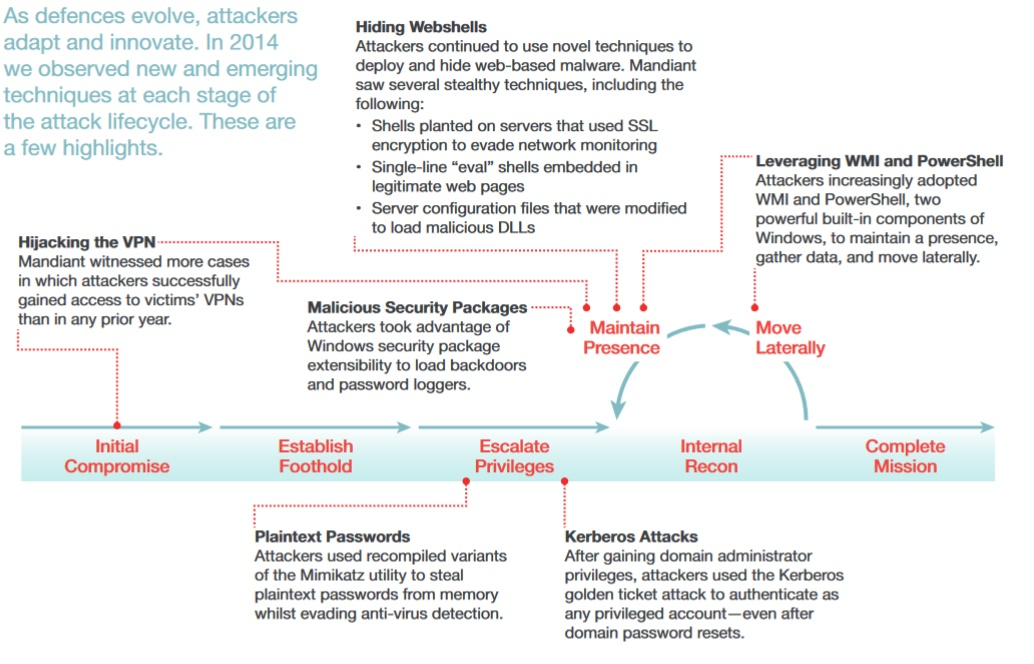
\includegraphics[scale=0.55]{AttackLifecycle.jpg}
 Advanced threat actors continue to evolve their tools and 
tactics to reduce the forensic footprint of their activities and evade detection. 
Targeted organisations need to ensure that they maintain capabilities for both 
real-time monitoring and “look-back” forensics capabilities across endpoint 
systems, log sources, and network devices. Establishing a baseline of normal activity 
in an environment, and proactively hunting for deviations from this baseline, are 
essential to stay a step ahead of intruder’s efforts.
\subsection{Blurred lines-criminal and APT actors take a page from each other's playbook}
 As the tools, techniques, and procedures of criminal and  
APT actors coalesce, you must scrutinise actors’ intent and motivations. Only  
then can you properly assess the potential impacts of security incidents, respond 
appropriately, and create a security strategy appropriate for the threats you face. 
\section{Conclusion}
Far too many organisations were unprepared for the inevitable breach, allowing attackers to linger far too long in compromised environments.\\
No one can prevent every breach. But by preventing, detecting, analysing, and responding to the most advanced threats quickly and effectively, you can protect yourself,
your customers, and your partners from the headline-generating consequences.
\chapter{McAfee Threats Report}
\section{Summary}...
\section{Key Reports}
\subsection{The equation group: hard disk and solid state drive firmware}
\subsection{Ransomware}
\subsection{Adobe Flash}
\section{Threat Statistics}
\chapter{Hacking human OS(social engineering)}
\section{Intro}
\section{Social engineering}
\section{Attacks}
\section{Attacks Lifecycle}
\section{Channels of attack}
\section{Defence ?}
\section{Conclusion}
\chapter{DPI (deep packet inspection) and data protection law}
\section{Confidentiality of communications (Art.5)(EUROPE)}
Member States shall ensure the  confidentiality of communications and the related traffic data. Meaning they have to prohibit listening, tapping, storage or other kinds of interception or  surveillance.
\section{Principle of erasure of traffic data (Art.6)}
\subsection{paragraph 1}
Traffic data relating to subscribers and users must be erased or made anonymous when it is no longer needed for the purpose of the transmission of a communication.\\
Traffic data =  any data processed for the purpose of the conveyance of a communication on an electronic communications network or for the billing thereof.
\subsection{paragraph 2-4 (exceptions)}
\begin{enumerate}
\item Traffic data necessary for the purposes of subscriber billing and interconnection payments may be processed 
\item Traffic data necessary for the purpose of marketing electronic communications services or for the provision of value added services may be processed but consent of users required.\\ Value added service = any service which requires the processing of traffic data or location data other than traffic data beyond what is necessary for the transmission of a communication or the billing thereof 
\end{enumerate}
\subsection{paragraph 5}
Processing of traffic data, in accordance with paragraphs 1, 2, 3 and 4, must be restricted to persons acting under the authority of providers of the public communications networks and publicly available electronic communications services handling billing or traffic management, customer enquiries, fraud detection, marketing electronic communications services or providing a value added service, and must be restricted to what is necessary for the purposes of such activities.\\ This means that is possible to process traffic data for traffic management purposes without users consent(NOT IN UK).
\section{Questions}
This raises an important question: If it is possible to process traffic data for traffic management and network security purposes : \\
\begin{enumerate}
\item How deep can you go? 
\item What can you do with the data? 
\item Can ISPs retain the data? 
\end{enumerate}
It would seem that the answer from the CJEU(Court of Justice of the European Union) is that the systematic retention of traffic data, location data and the related data necessary to identify the subscriber or user =  Interference with the right to respect for private life! This means this systematic retention is illegal ?
\chapter{From porn to cyber security passing by copyright: How mass surveillance technologies are gaining legitimacy... The case of Deep packet inspection technologies}
\section{Intro}
pervasive = spread throughout.\\
Monitoring of traffic data is becoming more and more common. This paper has 2 objectives that wants to discuss:\\
\begin{enumerate}
\item At the same rate people are becoming more aware of the power of the ISP's, DPI is gaining legal legitimacy.
\item Review European data protection laws and privacy rights to include the discussion of DPI.
\end{enumerate}
The pervasive monitoring by governments agencies and states has increased the interest in this field.\\
\textbf{Deep  Packet  Inspection} (DPI)  technologies  are  able  to  make  anything  that  happens  on  a  
network  visible  and  recordable. Therefore they can be considered as surveillance. If you consider all the traffic it might be impossible to analyse but if focused on specific patterns then we have to fear for privacy!!
\section{Types of DPI}

\section{Content regulation}
\subsection{Private experiments}
\subsection{EU framework}
\subsection{National interpretations}
\section{Data protection}
\subsection{The Lawful processing of personal data through the means of DPI(lawful = allowed or permitted by law)}
\subsection{The confinement of the processing of personal data through the means of DPI (confinement = hidding)}
\section{Conclusions}
\chapter{How To Break Anonymity of the Netflix Prize Dataset}
\section{Intro}
As part of the Netflix Prize contest, Netflix—the world’s largest online movie rental service—publicly released a dataset containing movie ratings of 500,000 Netflix subscribers. The dataset is intended to be anonymous, and all personally identifying information has been removed. They demonstrated that by crossing the data with the IMDB (Internet Movie DB) they were able to find the identities and therefore deanonymise the huge dataset.\\
What is more incredible is that what a person watches is really telling about the life of this person,  It’s like a self-portrait in movie titles: Nowhere else is cultural desire so nakedly on display.\\\\
The contest had the following specifications: 1M\$ for improving their movie recommendation service. To aid contestants, Netflix publicly released a dataset containing 100,480,507 movie ratings, created by 480,189 Netflix subscribers between December 1999 and December 2005.\\
Cases of deanonimyzation excited before showing that removing the identifying information isn't enough because with the help of auxiliary dataset the information could be reconnected.\\
The interesting \textbf{question} to ask is the following: How  much  does  the  attacker  need  to  know about a Netflix subscriber in order to identify her record in the dataset, and thus learn her complete movie viewing history. The answer is \textbf{VERY LITTLE}. This will be proven in the following arguments.
\section{Walkthrough the attacker mindset}
\section{Does privacy of Netflix ratings matter?}
The question asked isn't right, the right one is: Are there any Netflix subscribers whose privacy can be compromised by analyzing the Netflix Prize datase?\\
Interesting aspect, even if in the present this privacy breach might not seem important this can be studied as forward secrecy which can have hue impact in someone's future privacy! Plus even if this person creates anonymous virtual identities elsewhere, if any attacker is able to link the discovered data with the latter identity she won't be anonymous anymore.
\chapter{a firm foundation for Private Data analysis}
\section{Interesting points}
\begin{enumerate}
\item query monitoring is computationally infeasible and that the refusal to respond to a query may itself be disclosive.
\item In sub-sampling a subset of the rows is chosen at 
random and released.\\
\textbf{Does that means that sensitive data is disclosed in those sample ??} This questions comes from this comment: "Suppose appearing in a sub-sample has terrible consequences. Then every time sub-sampling occurs some individual suffers horribly.
\item In input perturbation, either the data or the queries are modified before a response is generated. This one is pretty good but "However, an outlier(donnée aberrante est une valeur ou une observation qui est "distante" des autres) may only be protected by the unlikelihood of being in the sub-sample". Does it mean that if you have a snignifical differene from the other data your only way to stay "privat" is not to be in the sub-sample?
\item Randomized response: Randomized response was devised for the setting in which the individuals do not trust the curator, so we can think of the randomized responses as simply being published. Privacy comes from the uncertainty  of how to interpret a reported value. The approach becomes untenable for complex data
\item Adding random noise to the output fails: suppose the noise has mean zero and that fresh randomness is used in generating every response. In this case, if the same query is asked repeatedly, then the responses can be averaged, and the true answer will eventually emerge.
\item Intro of differential privacy idea: What happens if the curator(Data curation is a broad term used to indicate processes and activities related to the organization and integration of data collected from various sources, annotation of the data, and publication and presentation of the data such that the value of the data is maintained over time, and the data remains available for reuse and preservation) permits only a sub-linear number of questions?\\\
\textbf{What is a sublinear number of questions ?} how to maintain privacy against a sub-linear number of counting  queries, that is, queries of the form “How many rows in the database satisfy property P ?” by adding noise of order less than the sampling error to each answer.
\item the importance of taking auxiliary information into account in privacy-preserving data release. 
\item auxiliary information to capture information about the respondents other than that which is obtained through the statistical database. Any priors, beliefs, or information from newspapers, labor statistics, and so on, all fall into this category.
\item Dalenius’s Desideratum: Anything that can be learned about a respondent from the statistical database should be learnable without access to the database. Which he was totally wrong unfortunately, simply explain the German height example.
\item New privacy goal: Minimize the increased risk to an individual incurred by joining (or leaving) the database. --> Solution: Differential Privacy!
\item differential privacy: Differential privacy will ensure that the ability of an adversary to inflict harm (or good, for that matter) of any sort, to any set of people should be essentially the same, independent of whether any individual opts in to, or opts out of, the dataset.
\end{enumerate}
\chapter{Breaking Diffie-Hellman}
\section{Technical aspect}
The Diffie Hellman was the system used for key exchange. The idea is that both parties want to communicate, but to do so thy need a common key to encrypt their messages. This key has to be known by both but can't be known by someone intercepting their messages, this is how it works: \\\\
Diffie-Hellman Protocol\\\\

The Diffie-Hellman protocol is a method for two computer users to generate a shared private key with which they can then exchange information across an insecure channel. Let the users be named Alice and Bob. First, they agree on two prime numbers g and p, where p is large (typically at least 512 bits) and g is a primitive root modulo p. (In practice, it is a good idea to choose $p$ such that $(p-1)/2$ is also prime.) The numbers $g$ and $p$ need not be kept secret from other users. Now Alice chooses a large random number a as her private key and Bob similarly chooses a large number b. Alice then computes $A=g^a (mod p)$, which she sends to Bob, and Bob computes $B=g^b (mod p)$, which he sends to Alice.\\\\

Now both Alice and Bob compute their shared key $K=g^(ab) (mod p)$, which Alice computes as\\
$K=B^a (mod p)=(g^b)^a (mod p)$\\\\

and Bob computes as\\
$K=A^b (mod p)=(g^a)^b (mod p)$.\\\\

Alice and Bob can now use their shared key $K$ to exchange information without worrying about other users obtaining this information. In order for a potential eavesdropper (Eve) to do so, she would first need to obtain $K=g^(ab) (mod p)$ knowing only $g$, $p$, $A=g^a (mod p)$ and $B=g^b (mod p)$.\\\\

This can be done by computing $a$ from $A=g^a (mod p)$ and $b$ from $B=g^b (mod p)$. This is the discrete logarithm problem, which is computationally infeasible for large $p$. Computing the discrete logarithm of a number modulo $p$ takes roughly the same amount of time as factoring the product of two primes the same size as $p$, which is what the security of the RSA cryptosystem relies on. Thus, the Diffie-Hellman protocol is roughly as secure as RSA. 
\section{Breaking}
Actually this part is less exciting, what happened is that many devices use the same key to communicate, therefore knowing this key would allow you to decrypt their messages pretty easily. The NSA realized that and decided to invest a lot of money and time to crack one of them, it is said that with their inversion they could possibly break 1 Key every year. When cracking the key, nothing was stopping them from eaves dropping any communication using that key. And the more time passes the more they can listen to. Unfortunately a lot of devices still use this method and it is really hard to change it.
\end{document}